\documentclass[14pt,a4paper,report]{report}
\usepackage[a4paper, mag=1000, left=2.5cm, right=1cm, top=2cm, bottom=2cm, headsep=0.7cm, footskip=1cm]{geometry}
\usepackage[utf8]{inputenc}
\usepackage[english,russian]{babel}
\usepackage{indentfirst}
\usepackage[dvipsnames]{xcolor}
\usepackage[colorlinks]{hyperref}
\usepackage{listings} 
\usepackage{fancyhdr}
\usepackage{caption}
\usepackage{graphicx}
\hypersetup{
	colorlinks = true,
	linkcolor  = black
}

\usepackage{titlesec}
\titleformat{\chapter}
{\Large\bfseries} % format
{}                % label
{0pt}             % sep
{\huge}           % before-code


\DeclareCaptionFont{white}{\color{white}} 

% Listing description
\usepackage{listings} 
\DeclareCaptionFormat{listing}{\colorbox{gray}{\parbox{\textwidth}{#1#2#3}}}
\captionsetup[lstlisting]{format=listing,labelfont=white,textfont=white}
\lstset{ 
	% Listing settings
	inputencoding = utf8,			
	extendedchars = \true, 
	keepspaces = true, 			  	 % Поддержка кириллицы и пробелов в комментариях
	language = bash,            	 	 % Язык программирования (для подсветки)
	basicstyle = \small\sffamily, 	 % Размер и начертание шрифта для подсветки кода
	numbers = left,               	 % Где поставить нумерацию строк (слева\справа)
	numberstyle = \tiny,          	 % Размер шрифта для номеров строк
	stepnumber = 1,               	 % Размер шага между двумя номерами строк
	numbersep = 5pt,              	 % Как далеко отстоят номера строк от подсвечиваемого кода
	backgroundcolor = \color{white}, % Цвет фона подсветки - используем \usepackage{color}
	showspaces = false,           	 % Показывать или нет пробелы специальными отступами
	showstringspaces = false,    	 % Показывать или нет пробелы в строках
	showtabs = false,           	 % Показывать или нет табуляцию в строках
	frame = single,              	 % Рисовать рамку вокруг кода
	tabsize = 2,                  	 % Размер табуляции по умолчанию равен 2 пробелам
	captionpos = t,             	 % Позиция заголовка вверху [t] или внизу [b] 
	breaklines = true,           	 % Автоматически переносить строки (да\нет)
	breakatwhitespace = false,   	 % Переносить строки только если есть пробел
	escapeinside = {\%*}{*)}      	 % Если нужно добавить комментарии в коде
}

\begin{document}

\def\contentsname{Contents}

% Titlepage
\begin{titlepage}
	\begin{center}
		\textsc{Peter the Great St.Petersburg Polytechnic University\\[5mm]
			Department of Computer Systems \& Software Engineering}
		
		\vfill
		
		\textbf{Laboratory report №5\\[3mm]
			Discipline: «Information Security»\\[3mm]
			Theme: «A free online service Qualys SSL Labs -- SSL Server Test»\\[41mm]
		}
	\end{center}
	
	\hfill
	\begin{minipage}{.4\textwidth}
		Made by student:\\[2mm] 
		Volkova M.D.\\
		Group: 13541/2\\[5mm]
		
		Lecturer:\\[2mm] 
		Bogach N.V.
	\end{minipage}
	\vfill
	\begin{center}
		Saint-Petersburg\\ \the\year\ y.
	\end{center}
\end{titlepage}

% Contents
\tableofcontents
\clearpage

\chapter{Laboratory work №5}

\section{Work purpose}

SSL Server Test performs a deep analysis of the configuration of any SSL web server on the public Internet.

\section{Task}

\subsubsection{Study}

\begin{enumerate}
	\item Learn how to deploy SSL/TLS correctly.
	\item Learn SSL security issues POODLE, HeartBleed.
\end{enumerate}

\subsubsection{Exercises}

\begin{enumerate}
	\item Choose one domain from a list of Recent Best and one from Recent Worst at SSL Server Test study reports and explain their summary
	\item Analyse a SSL-based domain:
	\begin{enumerate}
		\item Explain Summary
		\item Explain the abbreviations in Conguration
		\item Comment on Protocol Details
		\item Conclude about SSL status
	\end{enumerate}
\end{enumerate}

\clearpage

\section{Study}

\subsection{Learn how to deploy SSL/TLS correctly}

\subsubsection{Private Key and Certificate}

\begin{itemize}
	\item Use 2048-bit private keys
	\item Protect private key
	\begin{itemize}
		\item Generate private keys and certificate requests (CSRs) on the trusted computer.
		\item To prevent key compromise, use password protection.
		\item After compromising, revoke old certificates and generate new keys.
		\item Update certificates each year with new private keys.
	\end{itemize}
	\item Make sure you cover enough of the domain names you use.
	\item Obtain certificates from trusted certification authorities.
	\item Use reliable certificate signing algorithms.
\end{itemize}

\subsubsection{Configuration}

\begin{itemize}
	\item Configure the correct certificate chains (one certificate is not enough for one certificate)
	\item Use secure protocols. For example, TLS v1.0, v1.1 and v1.2
	\item Use secure encryption algorithms (for example symmetric with keys of at least 128 bits)
	\item Monitoring the selection of the encryption algorithm.
	\item Support Forward Secrecy - features a protocol that allows you to exchange data regardless of the private key of the server.
	\item Disable client security validation capabilities.
\end{itemize}

\subsubsection{Application Design}

\begin{itemize}
	\item Use HSTS (HTTP Strict Transport Security), a mechanism that activates the forced secure connection through the HTTPS protocol.
	\item Disable the caching for the important content from the content security cutoff point.
	\item Use protected cookies.
\end{itemize}

\subsection{Learn SSL security issues POODLE, HeartBleed}

\textbf{POODLE} --  is a vulnerability in SSLv3. The attacker sends data to the server on the SSL3 protocol from the changed target, which allows him to decrypt 1 byte for 256 requests. This is due to the fact that SSLV3 does not take into account the MAC address.

To implement a POODLE attack, you must:

\begin{itemize}
	\item Have the ability to listen and replace the attacker’s traffic
	\item Have the ability to make requests on behalf of the attacker with known attack text
\end{itemize}

\textbf{HeartBleed} -- s a security bug in the OpenSSL cryptography library, which is a widely used implementation of the Transport Layer Security (TLS) protocol. It allows unauthorized reading of memory on a server that may contain a variety of private data at this time.

\clearpage

\section{Exercises}

\subsection{Choose one domain from a list of Recent Best and one from Recent Worst at SSL Server Test study reports and explain their summary}

\subsubsection{Example one of the best report}

As an example of the best report, take a report on one of the https://github.com domain servers:

\begin{figure}[h!]
	\centering
	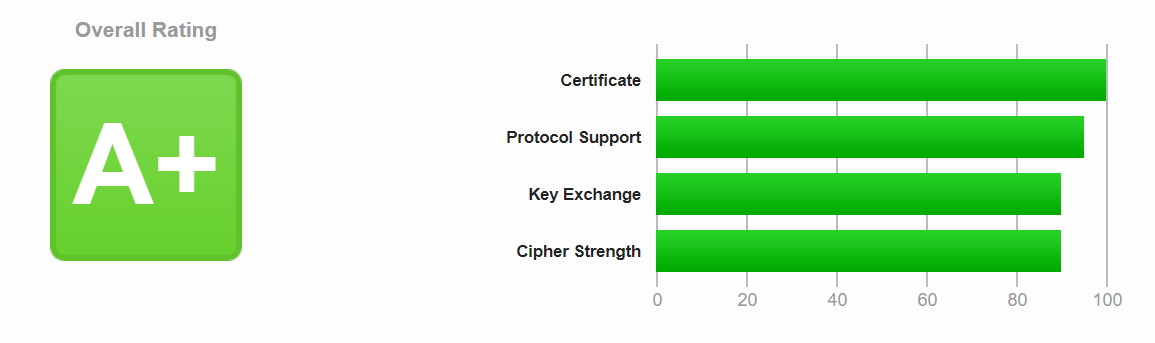
\includegraphics[scale = 0.50]{images/1.png}
	\caption{Summary of github.com analyze}
\end{figure}

\begin{figure}[h!]
	\centering
	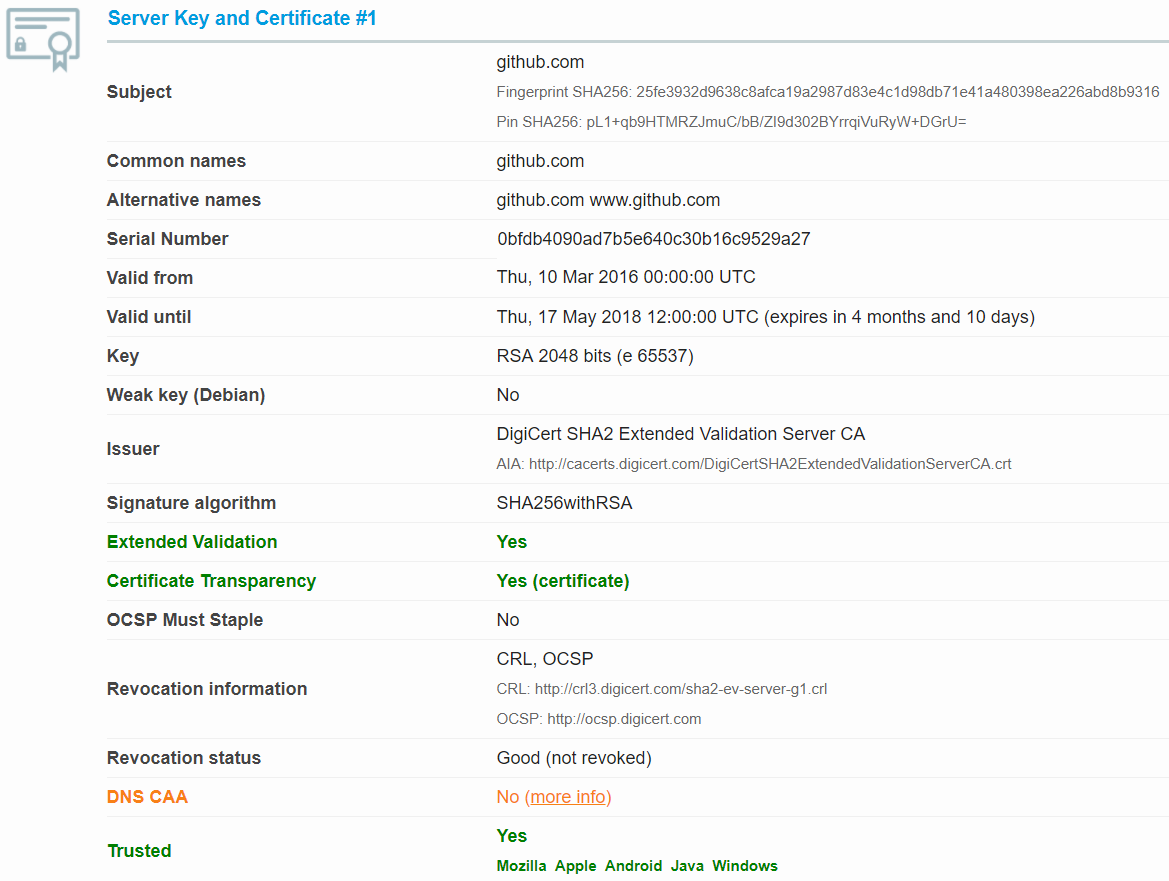
\includegraphics[scale = 0.53]{images/2.png}
	\caption{Server key and certificate of github.com domain}
\end{figure}

With this certificate there are practically no problems with any of the tests. We can be sure that the data of users of resource https://github.com can not be intercepted or replaced by an attacker.

\clearpage

\subsubsection{Example one of the worst report}

As an example of the best report, take a report on one of the http://spbstu.ru domain servers:

\begin{figure}[h!]
	\centering
	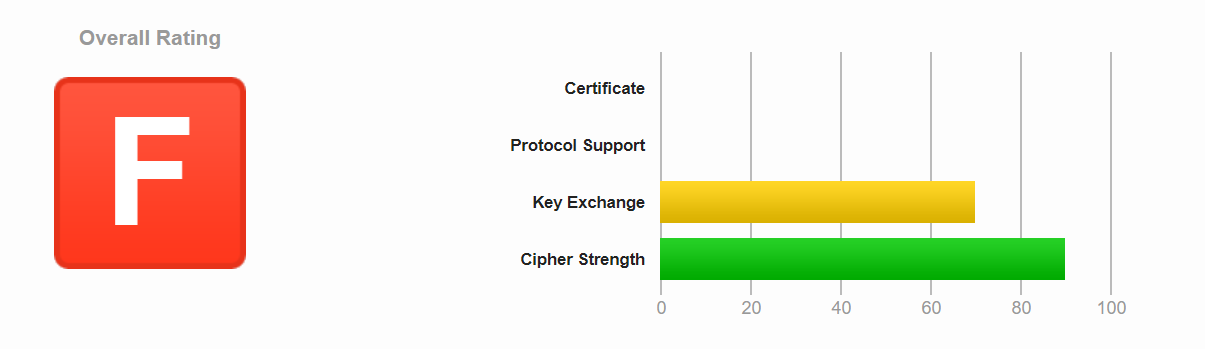
\includegraphics[scale = 0.50]{images/3.png}
	\caption{Summary of spbstu.ru analyze}
\end{figure}

\begin{figure}[h!]
	\centering
	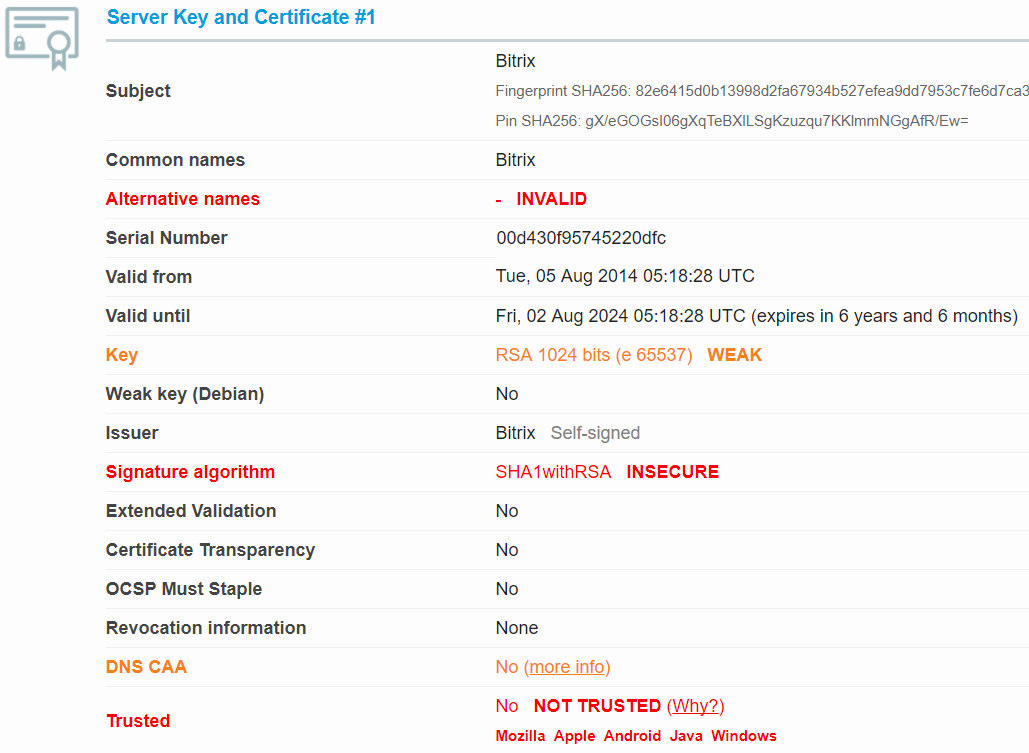
\includegraphics[scale = 0.61]{images/4.png}
	\caption{Server key and certificate of spbstu.ru domain}
\end{figure}

This certificate has several basic problems:

\begin{itemize}
	\item Not trusted and self signed.
	\item Weak encryption algorithm.
\end{itemize}

Data transmitted over the network can easily be intercepted by an attacker.

\subsection{Analyse a SSL-based domain}

\subsubsection{Explain Summary}

Server certificate is often the weakest point of an SSL server configuration. A certificate that is not trusted (i.e., is not ultimately signed by a well-known certificate authority) fails to prevent man-in-the-middle (MITM) attacks and renders SSL effectively useless. A certificate that is incorrect in some other way (e.g., a certificate that has expired) erodes trust and, in the long term, jeopardizes the security of the Internet as a whole.

For these reasons, any of the following certificate issues immediately result in a zero score:

\begin{itemize}
	\item Domain name mismatch.
	\item Certificate not yet valid.
	\item Certificate expired.
	\item Use of a self-signed certificate.
	\item Use of a certificate that is not trusted (unknown CA or some other validation error).
	\item Use of a revoked certificate.
	\item Insecure certificate signature (MD2 or MD5).
	\item Insecure key.
\end{itemize}

\subsubsection{Explain the abbreviations in Conguration}

\begin{itemize}
	\item TLS -- Transport Layer Security.
	\item SSL -- Secure Sockets Layer.
	\item RSA -- abbreviation for the names Rivest, Shamir and Adleman.
	\item RC4 -- Rivest cipher 4 or Ron’s code 4.
	\item SHA -- Secure Hash Algorithm.
	\item AES -- Advanced Encryption Standard.
	\item CBC -- Cipher Block Chaining.
	\item 3DES -- Triple Data Encryption Standard.
	\item SNI -- Server Name Indication
	\item NPN -- Next Protocol Negotiation.
	\item HSTS -- HTTP Strict Transport Security.
	\item HPKP -- HTTP Public Key Pinning.
	\item HTTP -- HyperText Transfer Protocol.
\end{itemize}

\subsubsection{Comment on Protocol Details}

\begin{itemize}
	\item \textbf{Secure Renegotiation} -- resuming TLS connection.
	\item \textbf{BEAST attack} -- attack by the BEAST utility (Browser Exploit Against SSL / TLS).
	\item \textbf{POODLE} is a vulnerability that allows you to decrypt the contents of a secure communication channel.
	\item \textbf{Downgrade attack} is an attack in which the user is forced to use less secure protocols that are still supported for compatibility reasons.
	\item \textbf{TLS compression} -- In 2012, CRIME attack showed how TLS compression can be used by attackers to identify details of sensitive data (for example, session cookies).
	\item \textbf{Heartbleed} -- an error in OpenSSL, which allows unauthorized reading of memory on the server up to 64 kilobytes per request. An attack can be made an infinite number of times.
	\item\textbf{Forward Secrecy} is a protocol feature that provides secure data exchange, it does not depend on the server’s private key. With encryption algorithms that do not support Forward Secrecy, it is possible to decrypt previously encrypted conversations using the private key of the server.
	\item \textbf{Next Protocol Negotiation} -- the client tells the server what protocols it would like to communicate with and the server can answer the most preferred one that it knows.
	\item \textbf{Strict Transport Security} -- a mechanism that activates the forced secure connection over HTTPS. This security policy allows you to immediately establish a secure connection, instead of using HTTP. The mechanism uses a special HTTP Strict-Transport-Security header to switch a user who has logged over HTTP to an HTTPS server.
\end{itemize}

\subsubsection{Conclude about SSL status}

The domain http://spbstu.ru has the rating "F" for the implementation of SSL. It's due to the following reasons:

\begin{itemize}
	\item Not trusted and self signed.
	\item Private key is not strong enough (RSA 1024 not enough to be secure in 2017);
	\item Vulnerability names OpenSSL Padding Oracle vuln.(CVE-2016-2107);
	\item Server supports weak Diffie-Hellman (DH) key exchange parameters.
\end{itemize}

The domain http://github.com has the rating "A+" for the implementation of SSL, because it is not subject to known vulnerabilities, trusted, and has a crypto-stable key length.

\section{Conclusion}

In this lab, we studied the «Qualys SSL Server Test» tool designed to test domains for the quality of the SSL/TLS encryption implementation. This resource provides an assessment of the quality of implementation based on many criteria and characteristics and then issues an assessment of the quality of implementation on its own scale of marks. It can be useful to identify unsafe resources on which your data can be stolen.




\end{document}